\documentclass[10pt]{beamer}
% \usepackage[utf8]{inputenc}

% FONTS
\usepackage[T1]{fontenc}
\usepackage{tgtermes}
\usepackage{amsmath}

% Font choice 2:
\usepackage[scaled=0.92]{PTSans}
\usepackage{amssymb}
\newcommand{\mathbold}[1]{\ensuremath{\boldsymbol{\mathbf{#1}}}}
\newcommand{\mbf}[1]{\ensuremath{\boldsymbol{\mathbf{#1}}}}

% \usepackage{lmodern}

%\usefonttheme{professionalfonts}

\usepackage{scalefnt,letltxmacro}
\LetLtxMacro{\oldtextsc}{\textsc}
\renewcommand{\textsc}[1]{\oldtextsc{\fontfamily{lmr}\scalefont{1}#1}}

% \renewcommand*\ttdefault{lmvtt}
\usepackage[ttdefault=true]{AnonymousPro}

% GEOMETRY
%\usepackage[
%  paper  = letterpaper,
%  left   = 1.65in,
%  right  = 1.65in,
%  top    = 1.0in,
%  bottom = 1.0in,
%  ]{geometry}

% # COLOR

% \usepackage[usenames,dvipsnames]{xcolor}
\definecolor{shadecolor}{gray}{0.9}

% \newcommand{\red}[1]{\textcolor{BrickRed}{#1}}
% \newcommand{\orange}[1]{\textcolor{BurntOrange}{#1}}
% \newcommand{\green}[1]{\textcolor{OliveGreen}{#1}}
% \newcommand{\blue}[1]{\textcolor{MidnightBlue}{#1}}
% \newcommand{\sky}[1]{\textcolor{SkyBlue}{#1}}
% \newcommand{\gray}[1]{\textcolor{black!60}{#1}}

% SPACING and TEXT
%\usepackage[final,expansion=alltext]{microtype}
\usepackage[english]{babel}
\usepackage[parfill]{parskip}
\usepackage{afterpage}
\usepackage{framed}
\usepackage{xspace}

% LEFTBAR
\renewenvironment{leftbar}[1][\hsize]
{%
  \def\FrameCommand
  {%
    {\color{Gray}\vrule width 3pt}%
    \hspace{10pt}%
    %\hspace{0pt}\fboxsep=\FrameSep\colorbox{black!10}%
  }%
  \MakeFramed{\hsize#1\advance\hsize-\width\FrameRestore}%
}%
{\endMakeFramed}

% EDITING
% line numbering in left margin
\usepackage{lineno}
\renewcommand\linenumberfont{\normalfont
                             \footnotesize
                             \sffamily
                             \color{SkyBlue}}
% ragged paragraphs in right margin
\usepackage{ragged2e}
% TODO should i rename sidenote marginpar?
\DeclareRobustCommand{\sidenote}[1]{\marginpar{
                                    \RaggedRight
                                    \textcolor{Plum}{\textsf{#1}}}}
% paragraph counter in right margin
\newcommand{\parnum}{\bfseries\P\arabic{parcount}}
\newcounter{parcount}
\newcommand\p{%
    \stepcounter{parcount}%
    \leavevmode\marginpar[\hfill\parnum]{\parnum}%
}
% pargraph header
\DeclareRobustCommand{\parhead}[1]{\textbf{#1}~}
% paragraph helper
\DeclareRobustCommand{\PP}{\textcolor{Plum}{\P} }

% COUNTERS
%\renewcommand{\labelenumi}{\color{black!67}{\arabic{enumi}.}}
%\renewcommand{\labelenumii}{{\color{black!67}(\alph{enumii})}}
%\renewcommand{\labelitemi}{{\color{black!67}\textbullet}}

% FIGURES
\usepackage{graphicx}
\usepackage[labelfont=bf]{caption}
%\usepackage[format=hang]{subcaption}

% TABLES
\usepackage{booktabs}

% # ALGORITHMS

\usepackage[algoruled]{algorithm2e}
\setlength{\interspacetitleruled}{8pt}
\usepackage{listings}
\usepackage{fancyvrb}
\fvset{fontsize=\small}

% HYPERREF
%\usepackage[colorlinks,linktoc=all]{hyperref}
%\usepackage[all]{hypcap}
\hypersetup{citecolor=Plum}
\hypersetup{linkcolor=MidnightBlue}
\hypersetup{urlcolor=MidnightBlue}

% CLEVEREF must come after HYPERREF
\usepackage[nameinlink]{cleveref}
\newcommand{\Crefb}[1]{(\Cref{#1})}
\newcommand{\crefb}[1]{(\cref{#1})}

% ACRONYMS
\usepackage[acronym,smallcaps,nowarn]{glossaries}
\glsdisablehyper
% \makeglossaries

% COLOR DEFINITIONS
\newcommand{\red}[1]{\textcolor{BrickRed}{#1}}
\newcommand{\orange}[1]{\textcolor{BurntOrange}{#1}}
\newcommand{\green}[1]{\textcolor{OliveGreen}{#1}}
\newcommand{\blue}[1]{\textcolor{MidnightBlue}{#1}}
\newcommand{\gray}[1]{\textcolor{black!60}{#1}}

% CODE
\usepackage{minted}  % for syntax highlighting

% REFERENCES
\usepackage[
  backend=biber,
  natbib,
  doi=false,isbn=false,url=false,
  sorting=none,
  citestyle=authoryear]{biblatex}

\newacronym{PPL}{ppl}{probabilistic programming language}
\newacronym{GPU}{\textnormal{\uppercase{gpu}}}{graphics processing unit}

\newacronym{VAE}{vae}{variational auto-encoder}
\newacronym{RBM}{rbm}{restricted Boltzmann machine}
\newacronym{DLGM}{dlgm}{deep latent Gaussian model}
\newacronym{GAN}{gan}{generative adversarial network}
\newacronym{RNN}{rnn}{recurrent neural network}

\newacronym{VI}{vi}{variational inference}
\newacronym{MCMC}{mcmc}{Markov chain Monte Carlo}
\newacronym{MC}{mc}{Monte Carlo}
\newacronym{HMC}{hmc}{Hamiltonian Monte Carlo}
\newacronym{MAP}{map}{maximum a posteriori}
\newacronym{IWAE}{iwae}{importance-weighted auto-encoder}
\newacronym{HVM}{hvm}{hierarchical variational model}
\newacronym{KL}{kl}{Kullback-Leibler}
\newacronym{ELBO}{elbo}{\emph{evidence lower bound}}

\DeclareRobustCommand{\mb}[1]{\ensuremath{\boldsymbol{\mathbf{#1}}}}

\newcommand{\mba}{\mathbold{a}}
\newcommand{\mbb}{\mathbold{b}}
\newcommand{\mbc}{\mathbold{c}}
\newcommand{\mbd}{\mathbold{d}}
\newcommand{\mbe}{\mathbold{e}}
%\newcommand{\mbf}{\mathbold{f}}
\newcommand{\mbg}{\mathbold{g}}
\newcommand{\mbh}{\mathbold{h}}
\newcommand{\mbi}{\mathbold{i}}
\newcommand{\mbj}{\mathbold{j}}
\newcommand{\mbk}{\mathbold{k}}
\newcommand{\mbl}{\mathbold{l}}
\newcommand{\mbm}{\mathbold{m}}
\newcommand{\mbn}{\mathbold{n}}
\newcommand{\mbo}{\mathbold{o}}
\newcommand{\mbp}{\mathbold{p}}
\newcommand{\mbq}{\mathbold{q}}
\newcommand{\mbr}{\mathbold{r}}
\newcommand{\mbs}{\mathbold{s}}
\newcommand{\mbt}{\mathbold{t}}
\newcommand{\mbu}{\mathbold{u}}
\newcommand{\mbv}{\mathbold{v}}
\newcommand{\mbw}{\mathbold{w}}
\newcommand{\mbx}{\mathbold{x}}
\newcommand{\mby}{\mathbold{y}}
\newcommand{\mbz}{\mathbold{z}}

\newcommand{\mbA}{\mathbold{A}}
\newcommand{\mbB}{\mathbold{B}}
\newcommand{\mbC}{\mathbold{C}}
\newcommand{\mbD}{\mathbold{D}}
\newcommand{\mbE}{\mathbold{E}}
\newcommand{\mbF}{\mathbold{F}}
\newcommand{\mbG}{\mathbold{G}}
\newcommand{\mbH}{\mathbold{H}}
\newcommand{\mbI}{\mathbold{I}}
\newcommand{\mbJ}{\mathbold{J}}
\newcommand{\mbK}{\mathbold{K}}
\newcommand{\mbL}{\mathbold{L}}
\newcommand{\mbM}{\mathbold{M}}
\newcommand{\mbN}{\mathbold{N}}
\newcommand{\mbO}{\mathbold{O}}
\newcommand{\mbP}{\mathbold{P}}
\newcommand{\mbQ}{\mathbold{Q}}
\newcommand{\mbR}{\mathbold{R}}
\newcommand{\mbS}{\mathbold{S}}
\newcommand{\mbT}{\mathbold{T}}
\newcommand{\mbU}{\mathbold{U}}
\newcommand{\mbV}{\mathbold{V}}
\newcommand{\mbW}{\mathbold{W}}
\newcommand{\mbX}{\mathbold{X}}
\newcommand{\mbY}{\mathbold{Y}}
\newcommand{\mbZ}{\mathbold{Z}}

\newcommand{\mbalpha}{\mathbold{\alpha}}
\newcommand{\mbbeta}{\mathbold{\beta}}
\newcommand{\mbdelta}{\mathbold{\delta}}
\newcommand{\mbepsilon}{\mathbold{\epsilon}}
\newcommand{\mbchi}{\mathbold{\chi}}
\newcommand{\mbeta}{\mathbold{\eta}}
\newcommand{\mbgamma}{\mathbold{\gamma}}
\newcommand{\mbiota}{\mathbold{\iota}}
\newcommand{\mbkappa}{\mathbold{\kappa}}
\newcommand{\mblambda}{\mathbold{\lambda}}
\newcommand{\mbmu}{\mathbold{\mu}}
\newcommand{\mbnu}{\mathbold{\nu}}
\newcommand{\mbomega}{\mathbold{\omega}}
\newcommand{\mbphi}{\mathbold{\phi}}
\newcommand{\mbpi}{\mathbold{\pi}}
\newcommand{\mbpsi}{\mathbold{\psi}}
\newcommand{\mbrho}{\mathbold{\rho}}
\newcommand{\mbsigma}{\mathbold{\sigma}}
\newcommand{\mbtau}{\mathbold{\tau}}
\newcommand{\mbtheta}{\mathbold{\theta}}
\newcommand{\mbupsilon}{\mathbold{\upsilon}}
\newcommand{\mbvarepsilon}{\mathbold{\varepsilon}}
\newcommand{\mbvarphi}{\mathbold{\varphi}}
\newcommand{\mbvartheta}{\mathbold{\vartheta}}
\newcommand{\mbvarrho}{\mathbold{\varrho}}
\newcommand{\mbxi}{\mathbold{\xi}}
\newcommand{\mbzeta}{\mathbold{\zeta}}

\newcommand{\mbDelta}{\mathbold{\Delta}}
\newcommand{\mbGamma}{\mathbold{\Gamma}}
\newcommand{\mbLambda}{\mathbold{\Lambda}}
\newcommand{\mbOmega}{\mathbold{\Omega}}
\newcommand{\mbPhi}{\mathbold{\Phi}}
\newcommand{\mbPi}{\mathbold{\Pi}}
\newcommand{\mbPsi}{\mathbold{\Psi}}
\newcommand{\mbSigma}{\mathbold{\Sigma}}
\newcommand{\mbTheta}{\mathbold{\Theta}}
\newcommand{\mbUpsilon}{\mathbold{\Upsilon}}
\newcommand{\mbXi}{\mathbold{\Xi}}

\renewcommand{\d}[1]{\ensuremath{\operatorname{d}\!{#1}}}
\newcommand{\g}{\,|\,}
\renewcommand{\gg}{\,\|\,}
\newcommand\dif{\mathop{}\!\mathrm{d}}
\newcommand{\diag}{\textrm{diag}}
\newcommand{\supp}{\textrm{supp}}
\newcommand{\Gam}{\textrm{Gam}}
\newcommand{\InvGam}{\textrm{InvGam}}
\DeclareMathOperator*{\argmax}{arg\,max}
\DeclareMathOperator*{\argmin}{arg\,min}
\DeclareRobustCommand{\KL}[2]{\ensuremath{\textrm{KL}\left(#1\;\|\;#2\right)}}
\newcommand\indep{\protect\mathpalette{\protect\independenT}{\perp}}
\def\independenT#1#2{\mathrel{\rlap{$#1#2$}\mkern2mu{#1#2}}}
\newcommand{\E}[1]{\mathbb{E}\left[ #1 \right]}

\usepackage{tikz}
\usetikzlibrary{bayesnet}

\pgfdeclarelayer{edgelayer}
\pgfdeclarelayer{nodelayer}
\pgfsetlayers{edgelayer,nodelayer,main}

\definecolor{hexcolor0xbfbfbf}{rgb}{0.749,0.749,0.749}

\tikzset{>=latex}
\tikzstyle{none}   = [inner sep=0pt]
\tikzstyle{line}   = [-,
                      thick,
                      shorten <=1pt,
                      shorten >=1pt]
\tikzstyle{arrow}  = [->,
                      thick,
                      shorten <=1pt,
                      shorten >=1pt]
\tikzstyle{ardash} = [dashed,
                      ->,
                      thick,
                      shorten <=1pt,
                      shorten >=1pt]

\tikzstyle{empty}=[
                   circle,
                   opacity=0.0,
                   text opacity=1.0,
                   inner sep=0pt
                  ]

\tikzstyle{box}=[
                 rectangle,
                 fill=White,
                 thick,
                 draw=Black,
                 inner sep=7pt
                ]

\tikzstyle{filled}=[
                    circle,
                    thick,
                    fill=hexcolor0xbfbfbf,
                    draw=Black
                   ]

\tikzstyle{hollow}=[
                    circle,
                    thick,
                    fill=White,
                    draw=Black
                   ]

\tikzstyle{param}=[
                   rectangle,
                   fill=Black,
                   draw=Black,
                   inner sep=0pt,
                   minimum width=4pt,
                   minimum height=4pt
                  ]

\tikzstyle{paramhollow}=[
                         rectangle,
                         thick,
                         fill=White,
                         draw=Black,
                         inner sep=0pt,
                         minimum
                         width=4pt,
                         minimum height=4pt
                        ]

\usepackage{pgfplots}                               % PGFPLOTS baby!
\pgfplotsset{compat=newest}
\pgfplotsset{plot coordinates/math parser=false}
% \usepgfplotslibrary{statistics}


\usetheme{simple}

\addbibresource{2017-04-Edward.bib}

% Watermark background (simple theme)
% \setwatermark{\includegraphics[height=8cm]{img/Heckert_GNU_white.png}}


\title{Probabilistic programming with Edward}
% \subtitle{}
\date{April 25, 2017}
\author{John Reid}
\institute{Biostatistics Unit, \\ School of Clinical Medicine, \\ Cambridge University}

\begin{document}

\maketitle

\begin{frame}
\frametitle{George E.P. Box (1919 - 2013)}
\begin{columns}
\begin{column}{0.4\textwidth}
    \begin{center}
     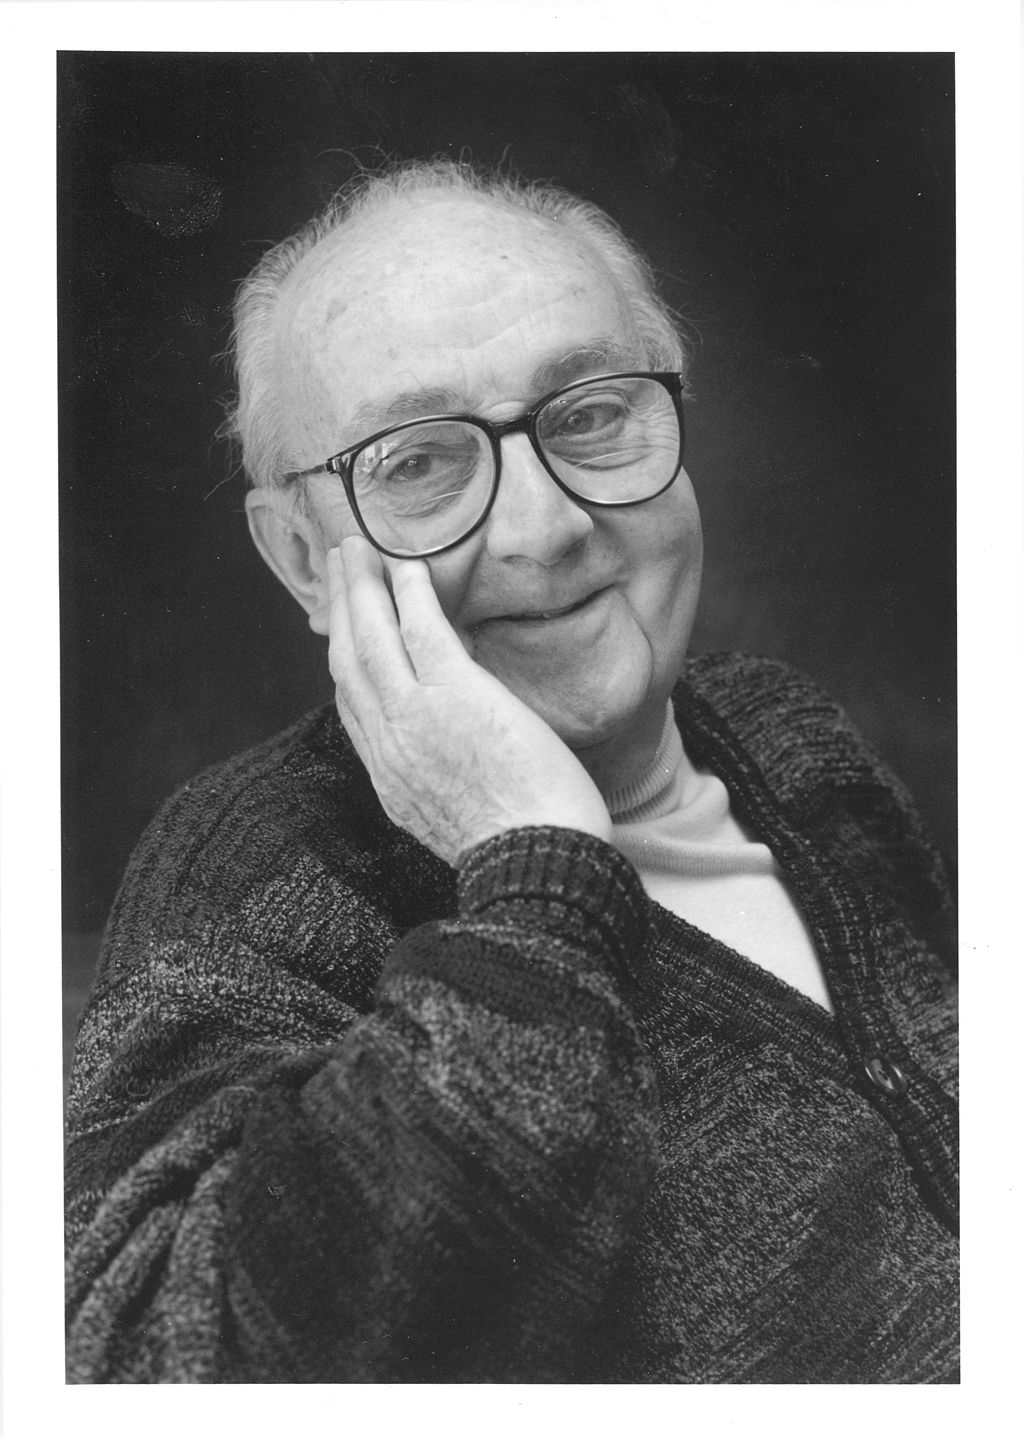
\includegraphics[width=\columnwidth]{img/box.jpg}
     \end{center}
\end{column}
\begin{column}{0.6\textwidth}
An iterative process for science:
\\[1ex]
\begin{enumerate}
\item Build a model of the science
\\[1ex]
\item Infer the model given data
\\[1ex]
\item Criticize the model given data
\end{enumerate}
\end{column}
\end{columns}
\citep{box_useful_1962-1, box_experimental_1965-1, box_discrimination_1967-1, box_science_1976-1, box_sampling_1980-1}
\end{frame}

\begin{frame}
\frametitle{Box's Loop}
\center
\begin{tikzpicture}[remember picture]
  \node [block] (Infer) {Infer};
  \coordinate[below of=Infer] (under);
  \node [block, left=of Infer] (Model) {Model};
  \draw [->, thick] (Model) -- (Infer);
  \node [block, right=of Infer] (Criticise) {Criticise};
  \draw [->, thick] (Infer) -- (Criticise);
  \draw [->, thick, rounded corners] (Criticise) -- (under) -- (Model);
  \node [block, above=of Infer, fill=blue!20] (Data) {Data};
  \draw [->, thick] (Data) -- (Infer);
\end{tikzpicture} \\
\vspace{20pt}
Edward is a library designed around this loop. \\
\citep{box_science_1976-1, box_sampling_1980-1, david_m._blei_build_2014}
\end{frame}


\begin{frame}
  \frametitle{Model comparisons}
  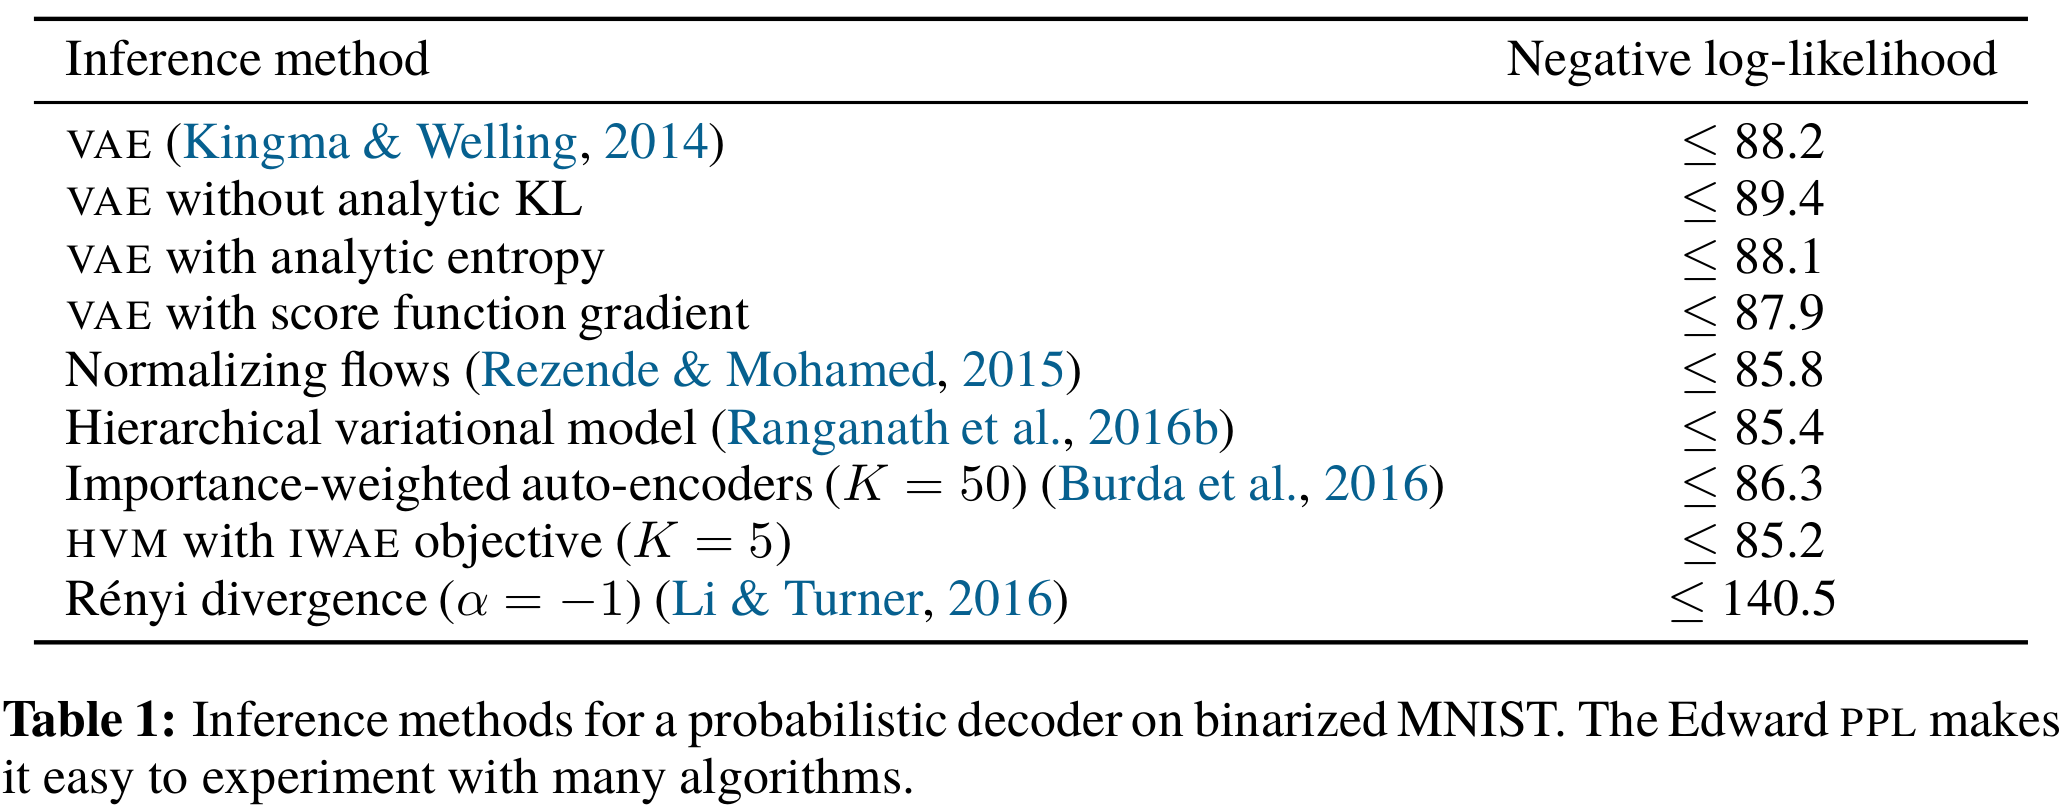
\includegraphics[width=\textwidth]{img/edward-lls.png}
\end{frame}


\begin{frame}
\vspace{3ex}
\textbf{Edward} is a probabilistic programming language,
designed for fast experimentation and research~\citep{tran_deep_2017}.

\emph{Modelling}
\begin{itemize}
\item Composable Turing-complete language of random variables.
\item Examples: Graphical models, neural networks, probabilistic programs.
\item Many data types, tensor vectorization, broadcasting, 3rd party support.
\end{itemize}

\emph{Inference}
\begin{itemize}
\item Composable language for hybrids, message passing, data subsampling.
\item Examples: Black box VI, Hamiltonian MC, stochastic gradient MCMC,
  generative adversarial networks.
\item Infrastructure to develop your own algorithms.
\end{itemize}

\emph{Criticism}
\begin{itemize}
\item Examples: Scoring rules, hypothesis tests, predictive checks.
\end{itemize}

\vspace{1ex}
Built on TensorFlow (features distributed computing, GPUs, autodiff).
\end{frame}

\begin{frame}[fragile]
\inputminted{python}{python/beta-bernoulli.py}
\end{frame}

\begin{frame}[fragile]
  \begin{block}{Model code}
    \begin{minted}{python}
      p = Beta(a=1.0, b=1.0)
      x = Bernoulli(p=tf.ones(10) * p)
    \end{minted}
  \end{block}
  The random variables $p$ and $x$ are represented by tensors $p^*$ and $x^*$ in the tensorflow computational graph
  \begin{block}{Computational graph}
    \begin{center}
      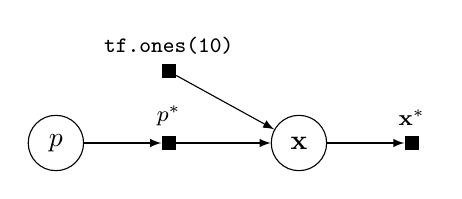
\begin{tikzpicture}[x=1.7cm,y=1.8cm,scale=0.9]
%\begin{tikzpicture}[scale=0.6]

  % Nodes
  \node[latent] (p) {$p$};
  \factor[right=of p, xshift=0.3cm] {thetastar} {$p^*$} {} {};

  \factor[above=of thetastar] {n} {\texttt{tf.ones(10)}} {} {};
  \node[latent, right=of thetastar, xshift=-0.5cm] (x) {$\mbx$};
  \factor[right=of x, xshift=0.3cm] {xstar} {$\mbx^*$} {} {};

  % Edges
  \edge{p}{thetastar};
  \edge{thetastar}{x};
  \edge{n}{x};
  \edge{x}{xstar};

\end{tikzpicture}

    \end{center}
  \end{block}
  Random variables are equipped with methods for likelihoods $\log(x|p)$,
  expectations $\mathbb{E}_{p(x|p)}[x]$, and sampling $\sim p(x|p)$.

  Graph can be executed by \mintinline{python}|x.value()| which returns the tensor $x^*$ and simulates the
  generative process.
\end{frame}


\begin{frame}[fragile]
  \frametitle{Model construction}
  Key concept is compositionality:
  \begin{itemize}
    \item Computational graphs can contain arbitrary tensorflow constructs
    \item Tensorflow conditional evaluations permit nonparametric processes
    \item Interface with third party tensorflow libraries, e.g. Keras for deep learning
  \end{itemize}
  \begin{block}{Deep generative model}
    \begin{minted}{python}
      from edward.models import Bernoulli, Normal
      from keras.layers import Dense

      z = Normal(mu=tf.zeros([N, d]), sigma=tf.ones([N, d]))
      h = Dense(256, activation='relu')(z.value())
      x = Bernoulli(logits=Dense(28 * 28)(h))
    \end{minted}
  \end{block}
\end{frame}


\begin{frame}
  \frametitle{Inference abstraction}
  Edward's random variables can represent probabilistic models as computational graphs.

  How to perform inference? We desire:
  \begin{itemize}
    \item Support for many inference classes
    \item The posterior can be further composed as part of a larger model
  \end{itemize}

  Edward abstracts this as an optimisation problem
  \begin{align*}
    \label{eq:inference-optimization}
    \min_{\mblambda,\mbtheta}
    \mathcal{L}(
      p(\mathbf{z} \mid \mathbf{x}; \mbtheta),
      q(\mathbf{z} ; \mbphi)
    )
  \end{align*}
  where $q$ can be a variational distribution, point estimate or collection of samples.

  The loss for the optimisation problem is encoded in the same computational graph as the model.
\end{frame}


\begin{frame}
  \frametitle{MNIST variational auto-encoder}
  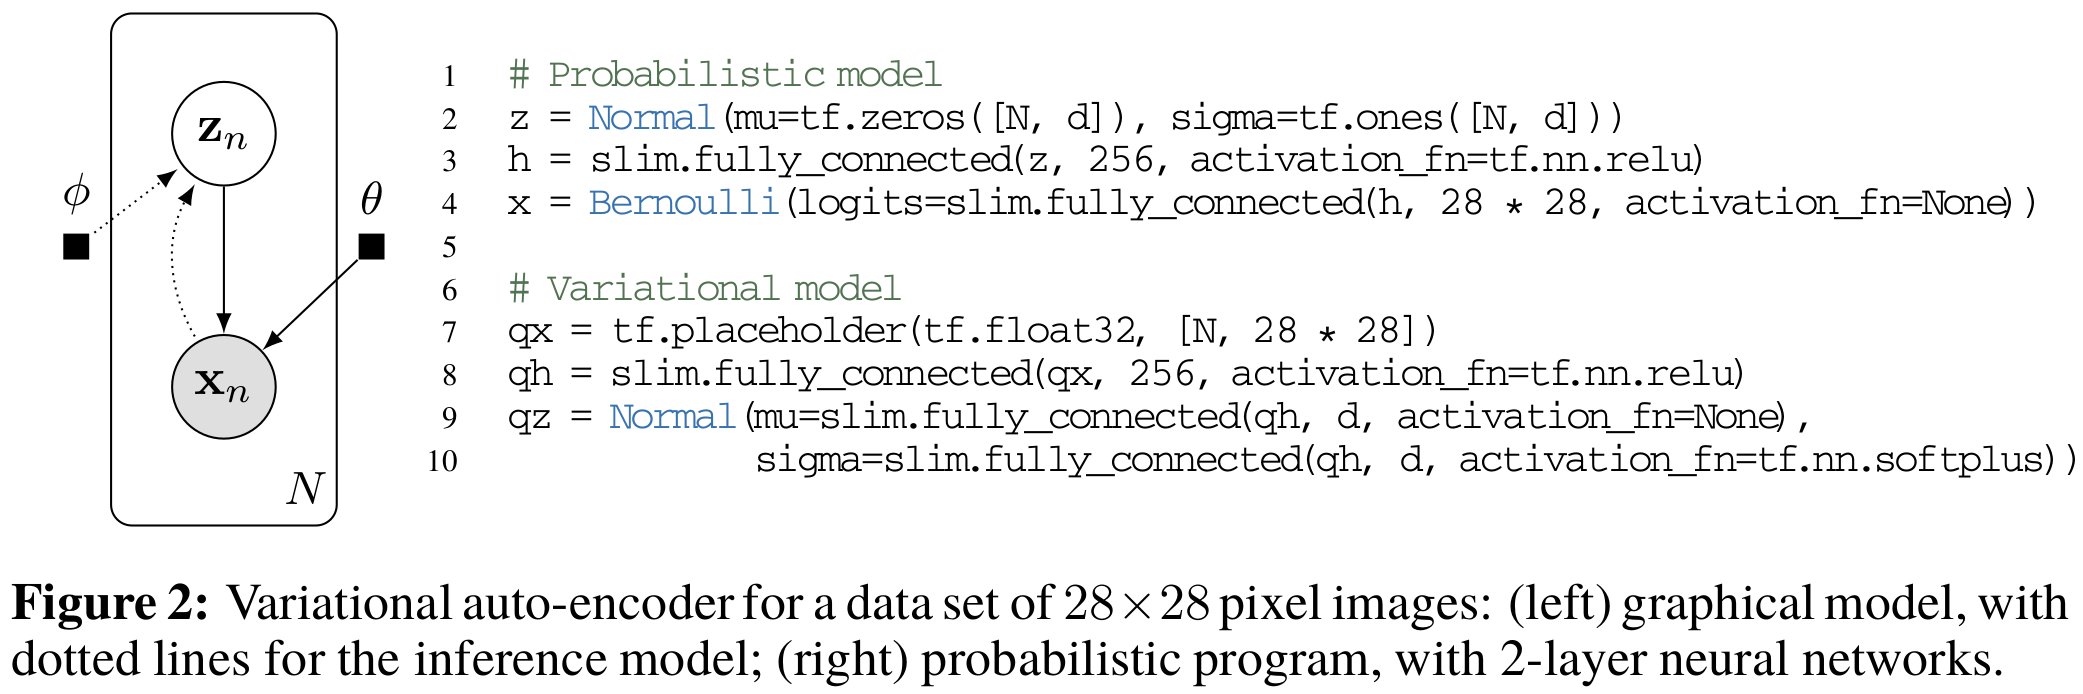
\includegraphics[width=\textwidth]{img/edward-vae.png}
\end{frame}


\begin{frame}
%  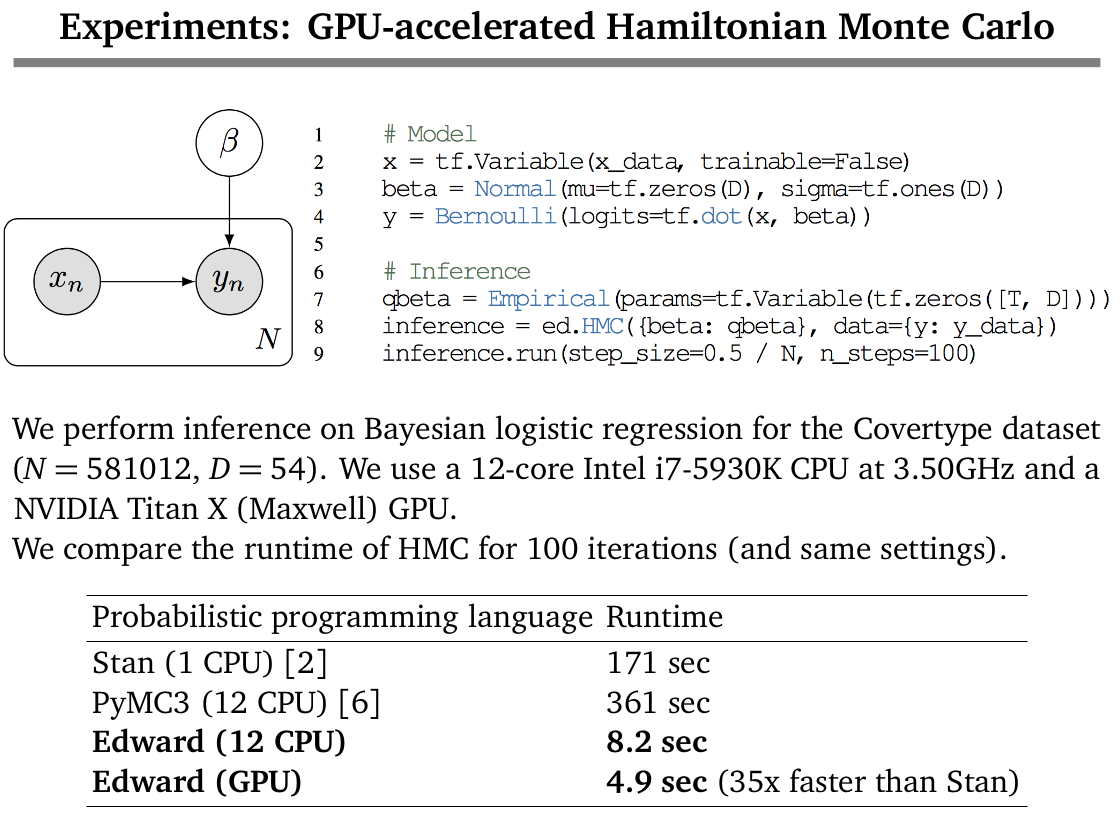
\includegraphics[width=\textwidth]{img/edward-GPU-speed.png}
\frametitle{GPU-accelerated Hamiltonian Monte Carlo}
\begin{tabular}{cc}
\hspace{-1em}
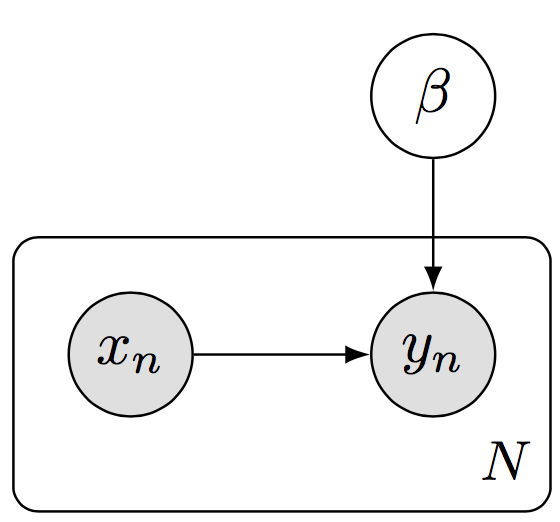
\includegraphics[width=2.5cm]{img/logistic_graph.png}
&
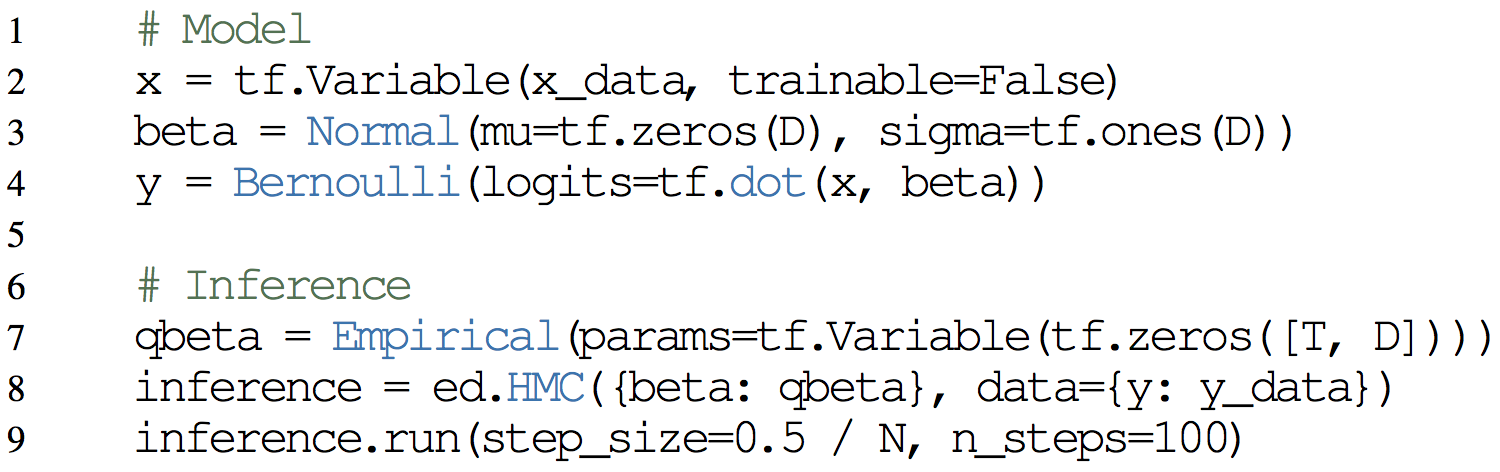
\includegraphics[width=7cm]{img/logistic_code.png}
\end{tabular}
\vspace{1ex}

Bayesian logistic regression for the Covertype dataset ($N=581012$, $D=54$) \\
12-core Intel i7-5930K CPU at 3.50GHz and a NVIDIA Titan X (Maxwell) GPU \\
100 iterations of HMC
\vspace{1ex}

\begin{table}[tb]
\centering
\begin{tabular}{ll}
\toprule
Probabilistic programming language & Runtime
\\
\midrule
Stan (1 CPU) & 171 sec \\
PyMC3 (12 CPU) & 361 sec \\
\textbf{Edward (12 CPU)} & \textbf{8.2 sec} \\
\textbf{Edward (GPU)} & \textbf{4.9 sec} (35x faster than Stan)\\
\bottomrule
\end{tabular}
\end{table}
\citep{carpenter_stan_2017, salvatier_probabilistic_2015}
\end{frame}



\begin{frame}
  \frametitle{Semi-supervised learning}

  \begin{columns}
    \begin{column}{0.4\textwidth}
      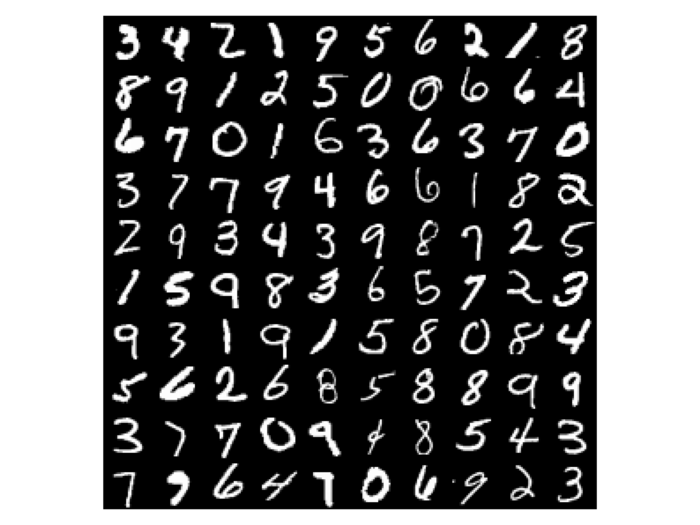
\includegraphics[width=\textwidth]{img/mnist-digits-small}
    \end{column}
    \begin{column}{0.6\textwidth}
      \begin{center}
        Model M2 from~\cite{kingma_semi-supervised_2014}
        \begin{align*}
          y &\sim \textnormal{Cat}(y|\pi) \\
          \mbz &\sim \mathcal{N}(0, I) \\
          \mbx|y, \mbz &\sim f(\mbx; y, \mbz, \theta)
        \end{align*}
        55,000 images, $\mbx$ \\
        3,000 have associated labels, $y$ \\
        $f$ is a deconvolutional network
      \end{center}
    \end{column}

  \end{columns}
\end{frame}



\begin{frame}
  \frametitle{Semi-supervised learning}

  posterior samples
\end{frame}



\begin{frame}
  \frametitle{}
\end{frame}



\begin{frame}
  \frametitle{}
\end{frame}


\begin{frame}[noframenumbering, allowframebreaks]  % in case more than 1 slide needed
  %\frametitle{References}
  \setbeamertemplate{bibliography item}[text]
  %\bibliographystyle{apalike}
  \renewcommand*{\bibfont}{\small}
  \printbibliography
\end{frame}
\end{document}
